\section{Theorie}
\label{sec:Theorie}
\subsection{Grundlagen der magnetischen Kernresonanz}
Die meisten Atomekerne besitzen neben Kernladung und Masse, auch einen Eigendrehimpuls, welcher als Spin $I$ bezeichnet wird.
Der Spin und das magnetische Dipolmoment des Atomkerns sind wie folgt miteinander verkn\"{u}pft:
\begin{align}
	\overrightarrow{\mu} = \hbar \gamma \overrightarrow{I}
\end{align}
hierbei ist $\gamma$ das gyromagnetische Verh\"{a}ltnis, welches element- und isotopenspezifisch ist.

In einem \"{a}u{\ss}eren Magnetfeld $\overrightarrow{B_0}$ richten sich die magnetischen Dipolmomente der Atomkern aus.
Klassisch betrachtet ist die Energie dann abh\"{a}ngig vom Relativwinkel zwischen $\overrightarrow{\mu}$ und $\overrightarrow{B_0}$.
In der quantenmechanischen Betrachtung sind jedoch nur bestimmte Winkel zugelasssen.
Erlaubt sind die Winkeleinstellungen, welche folgende Bedingung erf\"{u}llen:
\begin{align}
	E = -m \hbar \gamma_I B_0  \\
	\text{mit:} \, \, \,  m = +I, +(I-1), ..., -(I-1), -I
\end{align}
In einem \"{a}u{\ss}eren Magnetfeld befinden sich die Atomkerne somit auf verschiedenen Energieniveaus.
%- "Zeeman-Effekt"
Durch die unterschiedlichen Besetzungszahlen der einzelnen Niveaus kommt es zur  makroskopische Magnetisierung der Probe, dem Kernmagnetismus.
%- thermodynamischen Gleichgewicht Boltzmann-Verteilung
%- Kernmoment klein -> Ausrichtung durch externes Magnetfeld, Ausrichtung ist unab\"{a}ngig von der Orientierung der Molek\"{u}le

Zu der Ausrichtung kommt auf Grund des Drehimpulses eine Pr\"{a}zessionsbewegung dazu.
- Drehimpuls im Magnetfeld -> Pr\"{a}zessionsbewegung, diese ist senkrecht zum externen Magnetfeld, winkel zwischen $\mu$ und $B_0$ zeitlich konstant
- Lamorfrequenz: $\omega_0 = \gamma B_0$ hier: $\omega = 2\pi \cdot 90 \text{\, MHz}$
- wir betrachten die Summe aller Kernmomente: $M = \sum_i \mu_i$
- im Gleichgewicht ahebn alle die gleiche z-Komponente: $M = (0,0,M_z)$
- Gesamtmagnetisierung: $\frac{\vartheta M}{\vartheta t} = \gamma M_x B_0$
- $M und B_0$ sind parallel zueinander und damit zeitlich konstant
(- M kann auch pr\"{a}zidieren)

\paragraph{Rotierendes Koordinatensystem}
Da im folgenden senkrecht zu dem konstanten Magnetfeld ein zeitliches Hochfrequenzfeld (HF-Feld) $B_1(t)$ hinzugeschaltet wird, wird hier nun zun\"{a}chst das rotierende Koordinatensystem als Konzept eingef\"{u}hrt.
In solch einem rotierenden Koordinatensystem ergeben sich $B_0$ und $B_1(t)$ zusammen zu einem effektiven Magnetfeld $B_{eff}$.
Dreht sich die Z-Achse beispielsweise mit der Frequenz $\Omega$ um sich selbst, so gilt f\"{u}r die Gesamtmagnetisierung:
\begin{align}
	\frac{dM}{dt} = \gamma M \times B - \Omega \times M = \gamma M \times \left(B - \frac{\Omega}{\gamma} \right)
\end{align}
damit folgt f\"{u}r das effektive Magnetfeld:
\begin{align}
	\frac{dM}{dt} = \gamma M \times B_{eff} \, \Rightarrow \, B_{eff} = B - \frac{\Omega}{\gamma}
\end{align}
Somit wirkt das fiktive Feld $- \frac{\Omega}{\gamma}$ dem \"{a}u{\ss}eren Magnetfeld entgegen.

\begin{figure}[hbtp]
\centering
	\begin{subfigure}[c]{0.4\textwidth}
	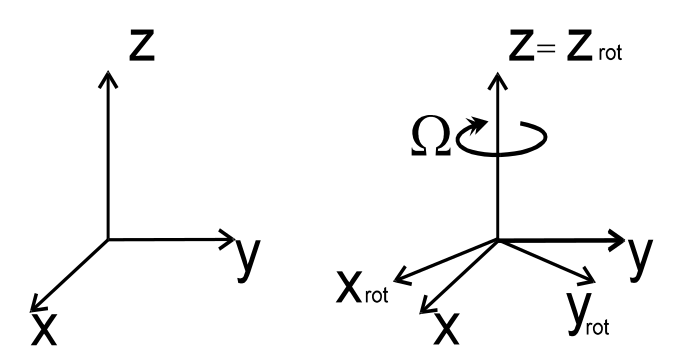
\includegraphics[width=\textwidth]{Plots/rotKoordinatensystem.png} 
	\subcaption{}
	\end{subfigure}
	~
	~
	\begin{subfigure}[c]{0.3\textwidth}
	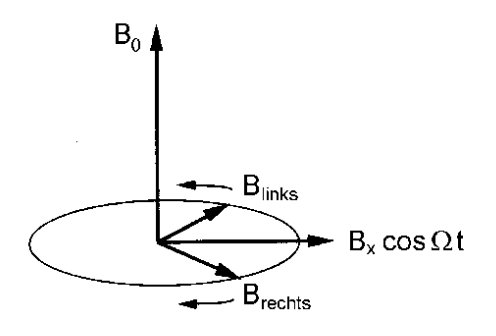
\includegraphics[width=\textwidth]{Plots/B1Felder.png}
	\subcaption{}
	\end{subfigure}
\caption{XXX}
\label{rotKoordi}
\end{figure}

Das Hochfrequenzfeld wir mit einer Spule erzeugt und ist im Labor gegeben durch:
\begin{align}
	B_1(t) = B_x cos(\Omega t)
\end{align}
Im rotierenden Koordinatensystem wird diese HF-Feld in eine linke $B_{1,\text{links}}$ und eine rechte $B_{1,\text{rechts}}$ Komponente aufgeteilt.
Beide Komponenten rotieren mit einer Frequenz von $|\Omega|$ und einer Amplitude von $\frac{B_x}{2}$.
Nun kann die Komponente, die sich mit dem Koordinatensystem rotiert, kann als station\"{a}r betrachtet werden.
Im Gegenschluss rotiert dann die andere Komponente mit $-2\Omega$ und ist im Allgemeinen vernachl\"{a}ssigbar.

\paragraph{Wirkungen von Hochfrequenzpulsen}
- wird aus einem kontinuierlichen Feld 'herausgeschnitten'
- HF-Puls, auch $90^{\circ}$-Puls oder $\frac{\pi}{2}$-Puls
- durch HF-Puls -> $\overrightarrow{\mu}$ macht viertel Drehung -> Quermagnetisierung
- beliebigen Winkel $\alpha$ einstellen: $\omega_1 = \frac{\alpha}{t_p} \Rightarrow t_p = \frac{2 \alpha}{\gamma B_x}$
- nach dem $90^{\circ}$-Puls: Pr\"{a}zession um $B_0$
- Pr\"{a}zession induziert Spannung in der Spule um die Probe -> Kerninduktionssignal
- Messung des Momentanwerts der L\"{a}ngsmagnetisierung
- Quermagnetisierung wird mit der Zeit kleiner
- effektive Quermagnetisierung dephasiert
- Rephasierung durch $180^{\circ}$-Puls
- Zusammentreffen der Signalpunkte = Hahn-Echo
- M im Hahn-Echo $\neq$ M nach $90^{\circ}$-Puls
- rotatorische und translatorische Molek\"{u}lbewegung -> Zerfall der Magnetisierung


\subsection{Relaxationen}
Die Magnetisierung $M(t)$ welche nach einen HF-Puls in der Probe vorliegt strebt wieder den Gleichgewichtswert $M_{eq}$ an.
Die Relaxation der Magnetisierung beruht auf der Wechselwirkung zwischen den Spins und deren Umgebung und wird in zwei Komponenten geteilt.
Zum Einen die longitudinale Relaxation entlang der z-Achse
\begin{align}
	\frac{d M_z(t)}{d t} = - \frac{M_z(t) - M_{eq}}{T_1}
\end{align}
und zum Anderen die transversale Relaxation in der x,y-Ebene
\begin{align}
	\frac{d M_{x,y}(t)}{d t} = - \frac{M_{x,y}(t)}{T_2} .
\end{align}
Diese beiden Gleichungen sind als Bloch-Gleichungen bekannt.
Dabei ist $T_1$ die Spin-Gitter-Relaxationszeit und $T_2$ die Spin-Spin-Relaxationszeit.
Im folgenden wird n\"{a}her auf die beiden Relaxationen eingegangen.

\paragraph{Spin-Gitter-Relaxation}
Die longitudinale Relaxation wird auch als Spin-Gitter-Relaxation bezeichnet.
Die dazugeh\"{o}rige $T_1$ Zeit kann mit der Inversionserholung gemessen werden.
Hierbei folgt auf einen $180^{\circ}$-Puls ein $90^{\circ}$-Puls.
\begin{figure}[hbtp]
	\centering
	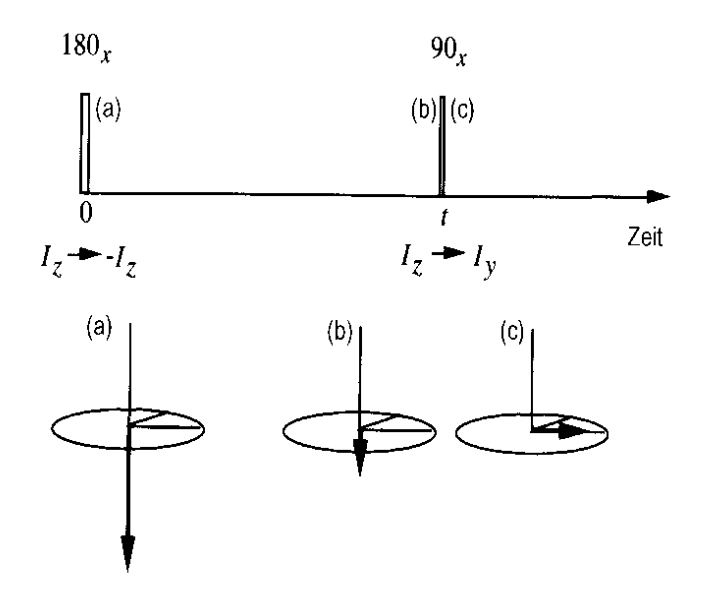
\includegraphics[width=0.4\textwidth]{Plots/inversionserholung.png}
	\caption{Pulsreihenfolge f\"{u}r eine Inversionserholung zur Messung der $T_1$-Zeit.}
	\label{inversion}
\end{figure}
Nach dieser Pulsreihenfolge zerf\"{a}llt die erzeugte Quermagnetisierung wieder und ein FID-Signal ist messbar.
Da die Amplitude dieses Signals proportiuonal zu der longitudinalen Magnetisierung ist, kann daraus dann die Relaxationszeit $T_1$ bestimmt werden.
Aus der ersten BLochgleichung kann die zeitabh\"{a}ngige longitudianle Magnetisierung ermittelt werden.
\begin{align}
	M_z(t) = M_{eq} \left(1 - 2 exp\left( - \frac{t}{T_1} \right) \right)
\end{align}
- f\"{u}r $t_{\frac{1}{2}} = T_1 \cdot ln(2)$ -> $M_z(t) = 0$
- um Sihnal-zu -Rauch-Verh\"{a}ltnis zu verbessern $t \approx 4 \cdot T_1$
- alternativ: S\"{a}ttigungserholung
- zerst\"{o}rung der Magnetisierung -> Wideraufbau der L\"{a}ngmagnetisierung -> Bestimmung von $T_1$
- mikroskopische Ursache der Spin-Gitter-Relaxation
- durch $180^{\circ}$-Puls -> Besetzungszinversion in energetisch ung\"{u}nstigen Zustand
-> $T_1$ -> Ma{\ss} f\"{u} die Effizient dieser \"{U}berg\"{a}nge
- spontane \"{U}berg\"{a}nge sehr unwahrscheinlich
- Emissionsprozesse m\"{u}ssen induziert werden -> durch magnetisches Wechselfeld
- Fluss von Energiequanten $(\hbar \omega_0)$ vom Kernspinsystem im Gitter

\paragraph{Spin-Spin-Relaxation}
- kein Energiefluss ins gitter
- Spin-Spin-WW -> Dipol-Dipol-WW
- WW zwischen Spins, also St\"{a}rke der Zusatzfelder abh\"{a}ngig von dem Winkel $\vartheta$, winkel zwischen $B_0$ und $r$
\begin{align}
	B_z^{DD} = \sum_s \hbar \gamma_s S \left( 3 cos^2 \left(\vartheta_{IS}\right) - 1 \right) \frac{1}{r_{IS}^3} \\
	B_{x,y}^{DD} = \sum_s \hbar \gamma_s S \left( \frac{3}{2} \cdot sin\left(2 \vartheta_{IS}\right) \right) \frac{1}{r_{IS}^3} \\
\end{align}
- $T_2$ immer kleiner als $T_1$
\begin{figure}[hbtp]
	\centering
	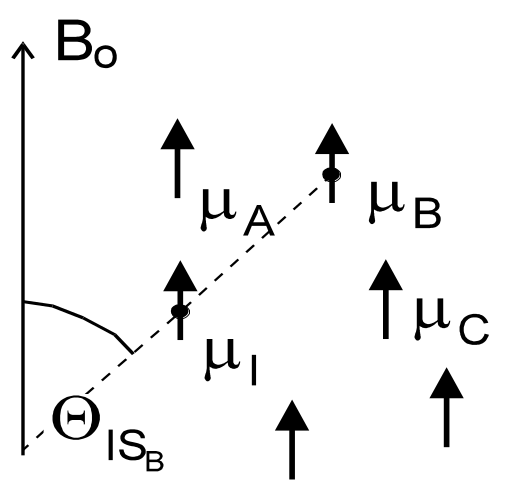
\includegraphics[width=0.5\textwidth]{Plots/spin_spin.png}
	\caption{Spin-Spin-Wechselwirkung.}
	\label{SpinSpin}
\end{figure}


\subsection{Hahn-Echo und Festk\"{o}rper-Echo}
1. Hahn-Echo
- f\"{u}r die Refokussierung von Wechselwirkungen, die linear in $\widehat{I}_z$ sind
- zum Beispiel: chemische Verschiebung, Dipol-Dipol-Wechselwirkung, Inhomogenit\"{a}ten von $B_{ext}$
-> mit $\widehat{H}_z = \omega \widehat{I}_z$
-> $90^{\circ}$-Puls und $180^{\circ}$-Puls
\begin{figure}[hbtp]
	\centering
	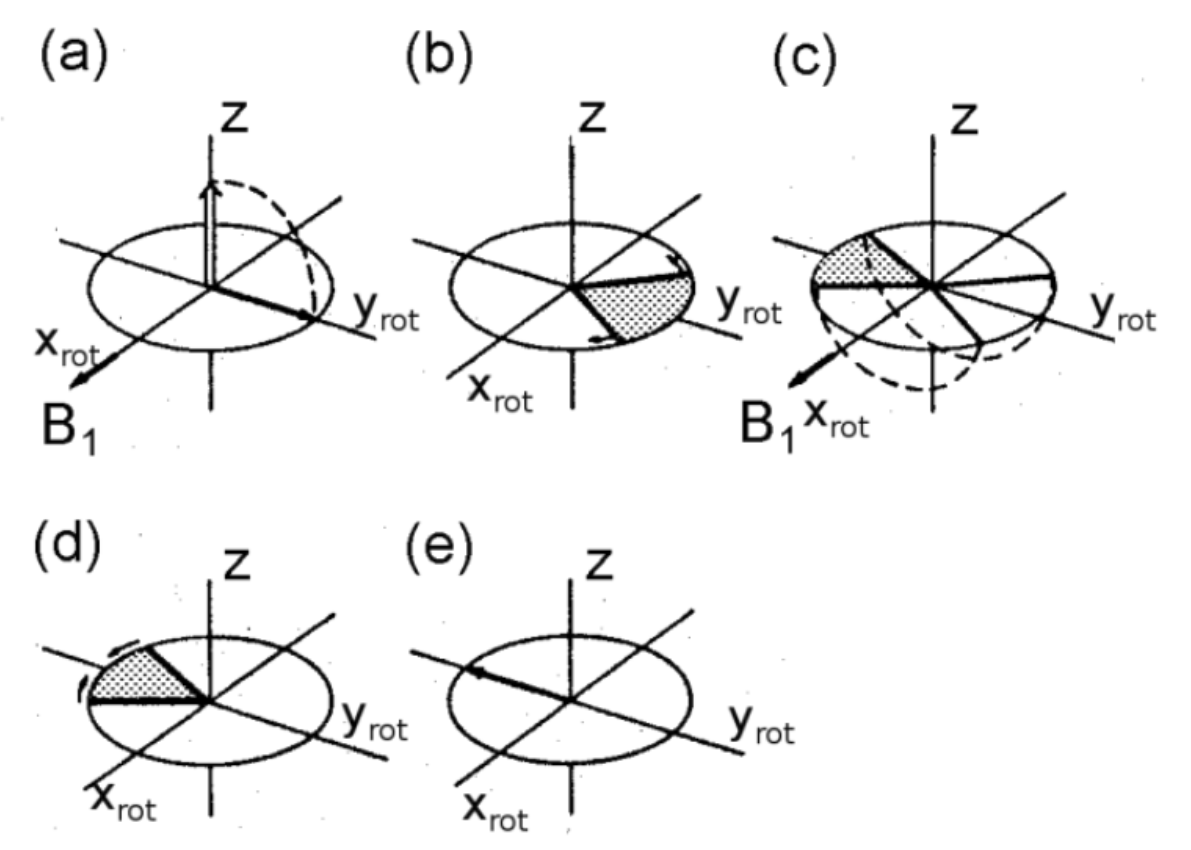
\includegraphics[width=0.5\textwidth]{Plots/hahnEcho.png}
	\caption{Hahn-Echo}
	\label{hahn}
\end{figure}


2. Festk\"{o}rper-Echo
- f\"{u}r die Refokussierung von Wechselwirkung die linear in homonuklearen Spinoperatoren 
-> $90^{\circ}$-Puls X und $90^{\circ}$-Puls, der um $\frac{\pi}{2}$ mit dem ersten Puls au{\ss}er Phase ist ($\pm Y$)
\begin{figure}
\centering
	\begin{subfigure}[b]{0.4\textwidth}
		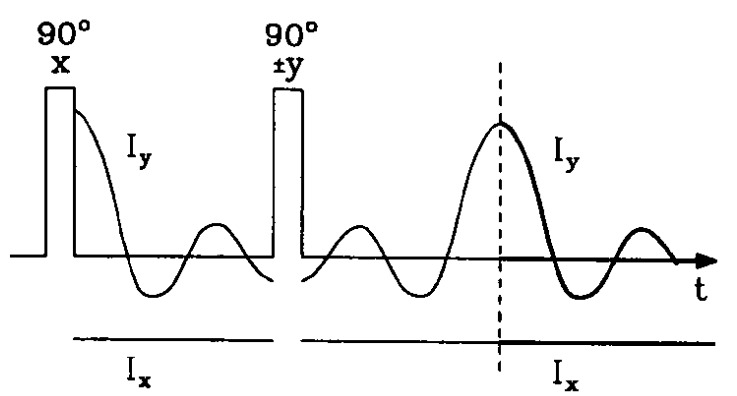
\includegraphics[width=\textwidth]{Plots/festkoerperecho.png}
		\caption{.}
		\label{.}
	\end{subfigure}
	~
	\begin{subfigure}[b]{0.4\textwidth}
		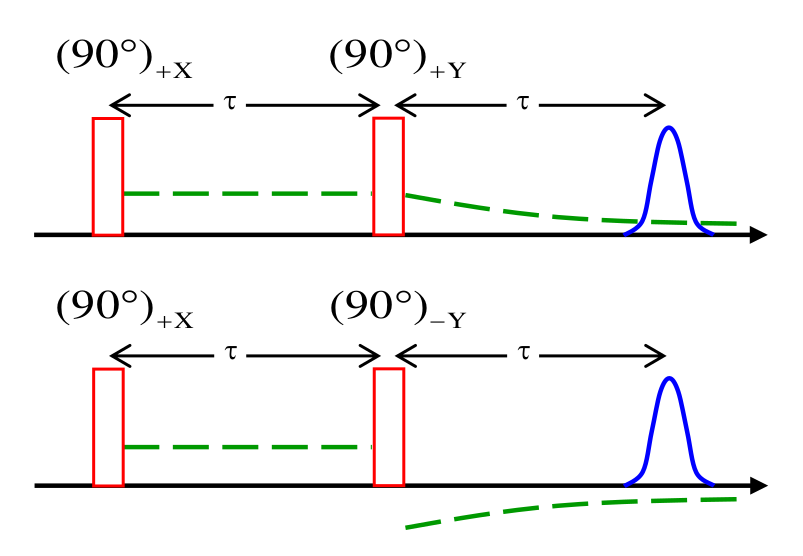
\includegraphics[width=\textwidth]{Plots/festkoerperecho2.png}
		\caption{.}
		\label{.}
	\end{subfigure}
\caption{Festk\"{o}rper-Echo}
\label{.}
\end{figure}


\subsection{Der $^2$H-Kernspin-Hamiltonoperator}
- aufspaltung
- Quadropolwechselwirkung
\begin{figure}[hbtp]
	\centering
	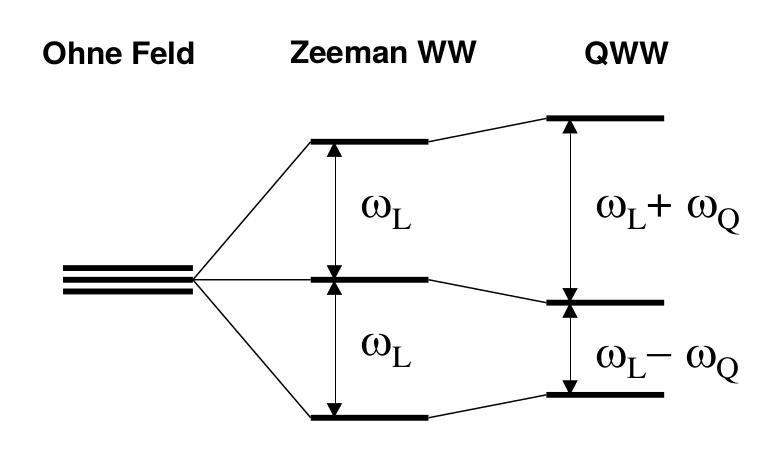
\includegraphics[width=0.4\textwidth]{Plots/aufspaltung.png}
	\caption{Aufspaltung}
	\label{}
\end{figure}



\subsection{Stimuliertes Echo}
-> Korrelationszeit
\begin{figure}
\centering
	\begin{subfigure}[b]{0.4\textwidth}
		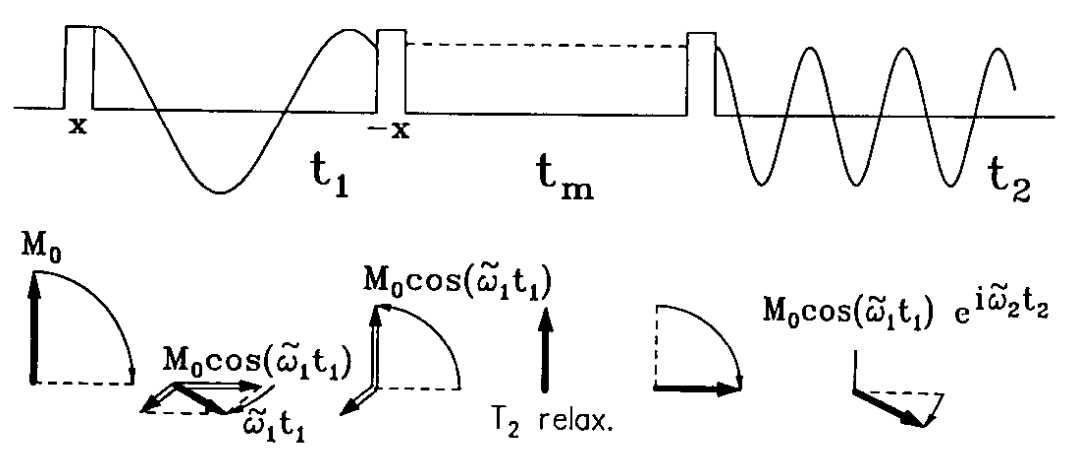
\includegraphics[width=\textwidth]{Plots/stimuliertesecho.png} 
		\caption{.}
		\label{.}
	\end{subfigure}
	~
	\begin{subfigure}[b]{0.4\textwidth}
		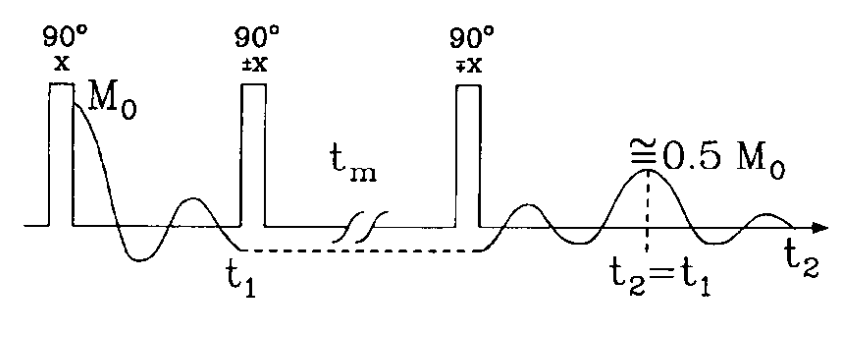
\includegraphics[width=\textwidth]{Plots/stimuliertesecho2.png}
		\caption{.}
		\label{.}
	\end{subfigure}
\caption{Festk\"{o}rper-Echo}
\label{.}
\end{figure}

\begin{figure}[hbtp]
	\centering
	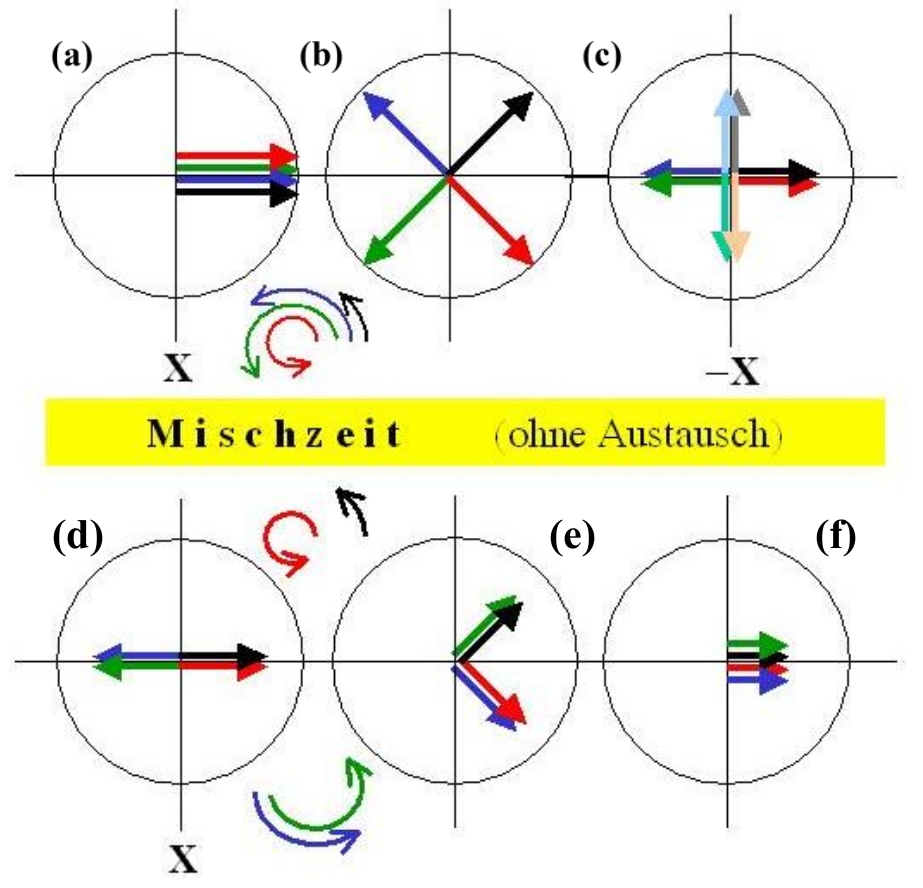
\includegraphics[width=0.5\textwidth]{Plots/mischzeit.png}
	\caption{.}
	\label{.}
\end{figure}
